\documentclass[10pt,a4paper]{article}
\usepackage[utf8]{inputenc}
\usepackage[T1]{fontenc}
\usepackage{listings}
\usepackage[english]{babel}
\usepackage{graphicx}
\usepackage[english]{isodate}
\usepackage[parfill]{parskip}
\usepackage{booktabs}
\usepackage{enumitem}
\usepackage[scaled=0.85]{beramono}


\usepackage{xcolor}

\colorlet{punct}{red!60!black}
\definecolor{background}{HTML}{EEEEEE}
\definecolor{delim}{RGB}{20,105,176}
\colorlet{numb}{magenta!60!black}

\lstdefinelanguage{json}{
    basicstyle=\scriptsize\ttfamily,
    numbers=left,
    numberstyle=\scriptsize,
    stepnumber=1,
    numbersep=8pt,
    showstringspaces=false,
    breaklines=true,
    frame=lines,
    backgroundcolor=\color{background},
    literate=
     *{0}{{{\color{numb}0}}}{1}
      {1}{{{\color{numb}1}}}{1}
      {2}{{{\color{numb}2}}}{1}
      {3}{{{\color{numb}3}}}{1}
      {4}{{{\color{numb}4}}}{1}
      {5}{{{\color{numb}5}}}{1}
      {6}{{{\color{numb}6}}}{1}
      {7}{{{\color{numb}7}}}{1}
      {8}{{{\color{numb}8}}}{1}
      {9}{{{\color{numb}9}}}{1}
      {:}{{{\color{punct}{:}}}}{1}
      {,}{{{\color{punct}{,}}}}{1}
      {\{}{{{\color{delim}{\{}}}}{1}
      {\}}{{{\color{delim}{\}}}}}{1}
      {[}{{{\color{delim}{[}}}}{1}
      {]}{{{\color{delim}{]}}}}{1},
}

\lstdefinelanguage{bash}{
    basicstyle=\normalfont\ttfamily,
    numbers=left,
    numberstyle=\scriptsize,
    stepnumber=10,
    numbersep=8pt,
    showstringspaces=false,
    breaklines=true,
    frame=lines,
    backgroundcolor=\color{background},
    literate=
     *{0}{{{\color{numb}0}}}{1}
      {1}{{{\color{numb}1}}}{1}
      {2}{{{\color{numb}2}}}{1}
      {3}{{{\color{numb}3}}}{1}
      {4}{{{\color{numb}4}}}{1}
      {5}{{{\color{numb}5}}}{1}
      {6}{{{\color{numb}6}}}{1}
      {7}{{{\color{numb}7}}}{1}
      {8}{{{\color{numb}8}}}{1}
      {9}{{{\color{numb}9}}}{1}
      {:}{{{\color{punct}{:}}}}{1}
      {,}{{{\color{punct}{,}}}}{1}
      {\{}{{{\color{delim}{\{}}}}{1}
      {\}}{{{\color{delim}{\}}}}}{1}
      {[}{{{\color{delim}{[}}}}{1}
      {]}{{{\color{delim}{]}}}}{1},
}

\title{TransitMapper Documentation \\ \large{\textbf{Draft}}}
\author{Patrick Brosi}

\begin{document}
\maketitle

\section{Basic Usage}

The input file is a graph given as a (simplified) Geo-JSON file, consisting of nodes (represented as ``Point''-features) and edges (represented as ``LineString''-features). Each edge has a collection of unique ``lines'' that travel through it. The transitmapper will render these lines in a way that resembles a transit map (Figure \ref{exampleoutput}). The input is read from \texttt{stdin}.

\begin{lstlisting}[language=bash,firstnumber=1]
$ transitmapper -o test.svg < test.json
\end{lstlisting}

See \ref{exampleinput} for an example input.

\begin{figure}[htbp]
  \centering
$	\vcenter{\hbox{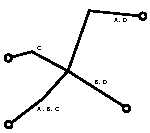
\includegraphics[width=0.36\textwidth]{inputex.pdf}}}$
	\hspace{5mm}
	$	\vcenter{\hbox{\scalebox{2}{\large $\Rightarrow$}}} $
	\hspace{5mm}
$	\vcenter{\hbox{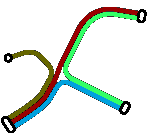
\includegraphics[width=0.36\textwidth]{test2.pdf}}}$
  \caption{Simple example output}
  \label{exampleoutput}
\end{figure}

\section{Command line parameters}

The following command line parameters are accepted by \texttt{transitmapper} (see also \texttt{-{}-help}).

\begin{description}[align=right]
	\item[\texttt{-{}-line-width=N}] The default width of a line, in output units. 20 by default.
	\item[\texttt{-{}-line-spacing=N}] The default spacing between lines, in output units. 10 by default.
	\item[\texttt{-{}-render-station-names}] Output the station names (experimental).
	\item[\texttt{-{}-render-node-fronts}] Output node fronts, useful for debugging.
	\item[\texttt{-{}-resolution=D}] Output resolution. 0.1 by default.
	\item[\texttt{-{}-no-optim}] (\texttt{-N}) Disable line-ordering optimization.
	\item[\texttt{-{}-input-smoothing=D}] Level of input-data smoothing. 3 by default.
\end{description}

\begin{figure}
  \centering
	$	\vcenter{\hbox{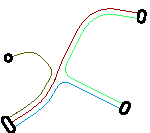
\includegraphics[width=0.36\textwidth]{test2_thin.pdf}}}$
	\hspace{5mm}
$	\vcenter{\hbox{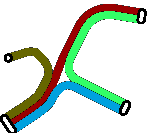
\includegraphics[width=0.36\textwidth]{test2_thick.pdf}}}$
	\caption{Different settings of \texttt{-{}-line-width} and \texttt{-{}-line-spacing}}
	\label{linewidths}
\end{figure}

\begin{figure}
  \centering
$	\vcenter{\hbox{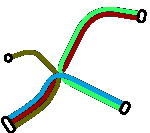
\includegraphics[width=0.36\textwidth]{test2_noopt.pdf}}}$
	\caption{Output without ordering optimization (\texttt{-N})}
  \label{wooptim}
\end{figure}

\begin{figure}
  \centering
$	\vcenter{\hbox{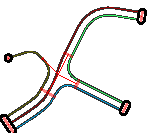
\includegraphics[width=0.36\textwidth]{test2_nodefronts.pdf}}}$
	\caption{Node-front rendering (\texttt{-{}-render-node-fronts})}
  \label{nodefronts}
\end{figure}

\begin{figure}
  \centering
$	\vcenter{\hbox{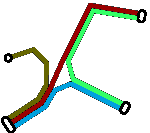
\includegraphics[width=0.36\textwidth]{test2_nosmoothing.pdf}}}$
	\caption{Without any line smoothing (\texttt{-{}-input-smoothing=0 -{}-bezier-prec=0})}
  \label{wosmoothing}
\end{figure}

\section{JSON Format}

See also ??. The input format is a lightweight subset of GeoJSON. At the top level, the input JSON must contain a \texttt{FeatureCollection} object:


\begin{lstlisting}[language=json,firstnumber=1]
{
  "type": "FeatureCollection",
  "features": [...]
}
\end{lstlisting}

A \texttt{feature} can either be a node (a \texttt{point}) or an edge (a \texttt{LineString}).

\subsection{Nodes}

A node consists of a geometry (the node's coordinates) and some properties.

\begin{lstlisting}[language=json,firstnumber=1]
{
  "geometry": {
	"coordinates": [0, 0],
	"type": "Point"
  },
  "properties": {
	"id": "1",
	"station_id": "1"
  }
}
\end{lstlisting}

\texttt{Type} is always \texttt{"point"}. The \texttt{coordinates} are given as an \texttt{[x,y]} array.

\subsubsection{Node Properties}

\begin{description}[align=right]
  \item[\texttt{id}] A dataset-unique string identifier for this node. Will be referenced later in edges.
  \item[\texttt{station\_id}] If this node is a station, the station's unique id (optional).
  \item[\texttt{station\_label}] If this node is a station, the station's name (optional). Either \texttt{station\_id} or \texttt{station\_label} has to be set for a node to become a station.
  \item[\texttt{excluded\_line\_conns}] A list of lines that are not connected in this node, even though two or more edges containing the line start/end in the node (Figure \ref{excllines}). The \texttt{line\_id} as well as the two edges this line is not connected in has to be given. Both edges are identified by the adjacent node. Example:
\begin{lstlisting}[language=json,firstnumber=1]
"excluded_line_conns": [
  {
	"edge1_node": "2",
	"edge2_node": "3",
	"route": "A"
  },
  {
	"edge1_node": "4",
	"edge2_node": "6",
	"route": "B"
  }
]
\end{lstlisting}

\begin{figure}
  \centering
$	\vcenter{\hbox{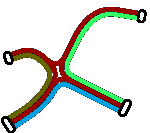
\includegraphics[width=0.36\textwidth]{test3.pdf}}}$
	\caption{The red line is not connected between the two main axes (via \texttt{exluded\_line\_connections})}
	\label{excllines}
\end{figure}

\end{description}

\subsection{Edges}

An edge consists also of a geometry (a linestring) and some properties.

\begin{lstlisting}[language=json,firstnumber=1]
{
  "geometry": {
	"coordinates": [
	  [0, 0], [500, 900], [1000, 950]
	],
	"type": "LineString"
  },
  "properties": {
	"from": "1",
	"to": "2",
	"lines": [
	  {"color": "00a1de"},
	  {"color": "990000"}
	]
  }
}
\end{lstlisting}


\subsubsection{Edge Properties}

Fields \texttt{from} and \texttt{to} hold the IDs of the nodes this edges connects. Property \texttt{lines} holds the lines that occur on that edge.

\begin{description}[align=right]
  \item[\texttt{from}] Holds the ID of the node this edge originates from.
  \item[\texttt{to}] Holds the ID of the node this edge ends in.
  \item[\texttt{lines}] An array of line objects, see below.
\end{description}

\subsubsection{Line object}

A line object is a single line occurance on an edge. Lines can either be identified accross edges by a unique ID or by the lines color as a shortcut. If you give a line an ID, you don't have to re-define its attributes again for an occurance in another edge. A single definition is enough.

The following properties are available for line occurances at the moment:

\begin{description}[align=right]
	\item[\texttt{id}] (optional) A unique string-identifier of this line. Will not be visible in the rendered output.
	\item[\texttt{label}] (optional) A string label that will be visible in the output as a line marker, if configured. Defaults to \texttt{""}.
	\item[\texttt{color}] (optional) The color this line will be rendered in, as a hexadecimal string (for example, \texttt{"660000"}. \textbf{Important:} if the line has no id, the color will be used for matching lines in adjacent edges.
	\item[\texttt{direction}] (optional) You may want to define a line that only occurs in one direction on the edge. This field allows you to specifiy the ID of the node this line is headed to. Node can either be \texttt{from} or \texttt{to}. \textbf{Note:} may be changed to a binary parameter. Defaults to a line that occurs in both directions. A single-direction line will be rendered with a little arrow indicating the direction. (Figure \ref{directedline}.)
	\item[\texttt{style}] (optional) A style attribute (still experimental). See below.
\end{description}

\subsubsection{Style object}

The style object can be used to define additional styles for lines. A style definition only changes the look of a line in the edge it is listed in. It is not global.

\begin{description}[align=right]
	\item[\texttt{dash-array}] (optional) A comma- or space-separated list of doubles. Starting at 1, the uneven positions are the lengths of filled line segments, the even positions are the lengths of the gaps. For example, \texttt{5, 10} produced a dashed line with segments of length 5, spaced by 10 units. (Figure \ref{dasharray}.)
	\item[\texttt{line-width}] (optional, \textbf{not yet implemented}) Overrides the width for this line, on this edge.
	\item[\texttt{line-spacing}] (optional, \textbf{not yet implemented}) Overrides the spacing for this line, on this edge.
	\item[\texttt{css}] (optional, \textbf{experimental!, only works with SVG output}) A free-hand css style for this line. Will be handed directly to the SVG renderer. The CSS defined here is not by the transitmapper to calculate spacing or optimize placements. For example, if you increase the width here, the line will overlap other lines.
\end{description}

\begin{figure}
  \centering
$	\vcenter{\hbox{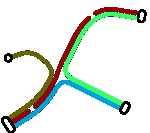
\includegraphics[width=0.36\textwidth]{test4.pdf}}}$
	\caption{Directed line (via \texttt{direction})}
  \label{directedline}
\end{figure}

\begin{figure}
  \centering
$	\vcenter{\hbox{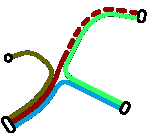
\includegraphics[width=0.36\textwidth]{test_dashed.pdf}}}$
	\caption{Line with \texttt{dash-array = "10 5"}}
  \label{dasharray}
\end{figure}

\section{Example Input}
\label{exampleinput}


\begin{lstlisting}[language=json,firstnumber=1]
{
  "type": "FeatureCollection",
  "features": [
    {
      "geometry": {
        "coordinates": [0, 0],
        "type": "Point"
      },
      "properties": {
        "id": "1",
        "station_id": "1"
      }
    },
    {
      "geometry": {
        "coordinates": [1000, 1000],
        "type": "Point"
      },
      "properties": {
        "id": "2",
        "station_id": "2"
      },
      "type": "Feature"
    },
    {
      "geometry": {
        "coordinates": [
          [0, 0], [500, 900], [1000, 950]
        ],
        "type": "LineString"
      },
      "properties": {
        "from": "1",
        "to": "2",
        "lines": [
          {"color": "00a1de"},
          {"color": "990000"}
        ]
      }
    }
  ]
}
\end{lstlisting}
\end{document}
